\section{Kameramodul Pixy (CMUcam5)}
\label{anhang-pixy}
Pixy ist ein schneller Bildsensor, welcher Objekte erkennen kann und das Resultat (Position/Fläche) an einen beliebigen Controller sendet.

Bildsensoren sind sehr flexibel, haben jedoch den Nachteil dass grosse Datenmengen anfallen und ein starker Prozessor für die Berechnung der Algorithmen benötigt wird. Pixy umgeht dieses Problem indem es einen Bildsensor mit einem Prozessor kombiniert. Pixy verarbeitet die Bilder vom Bildsensor und schickt die relevanten Informationen an den Controller (z.B. Raspberry Pi).

\subsection{Eckdaten}

\begin{itemize}
	\item Prozessor: NXP LPC4330, 204 MHz, dual core
	\item Bild Sensor: Omnivision OV9715, 1/4", 1280x800
	\item Framerate: 50Hz
	\item Sichtfeld: 75° horizontal (auf 2m Abstand 3m Sicht), 47° vertikal (auf 2m Abstand 1.7m Sicht)
	\item Linsen Typ: standard M12 (several different types available)
	\item Stromverbrauch: 140 mA (typisch)
	\item Spannung: 5V (bis zu 10V)
	\item RAM: 264K bytes
	\item Flash: 1M bytes
	\item Verfügbare Schnittstellen: UART serial, SPI, I2C, USB, digital, analog
	\item Abmessungen: 5.3cm x 4.4cm x 3.5cm
\end{itemize}

\subsection{Objekterkennung}

Pixy berechnet den Farbton und die Sättigung von jedem RGB-Pixel und filtert so das gewünschte Objekt heraus. Der Algorithmus ist robust gegen Lichtveränderungen (laut Hersteller). Ein Objekt kann in Pixy per Knopfdruck eingelernt werden. Es können bis zu 7 Objekte eingelernt werden.

\subsection{PixyMon}

PixyMon ist die Konfigurationssoftware für Pixy. Verbindet man seinen Laptop per USB-Kabel mit Pixy erhält man in PixyMon eine Liveansicht der Bilder (gut für Debbuging).

\subsection{Schnittstelle}

Alle 20ms sendet Pixy eine Liste von \textit{Object Blocks} über die serielle Schnittstelle (UART, SPI, I$^2$C) an den Controller. Die Object Blocks werden nach Objektgrösse sortiert. Der Aufbau des Blockes kann der unteren Abbildung entnommen werden.

\begin{figure}[h!]
\centering
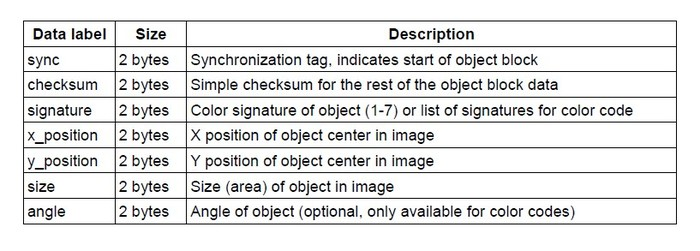
\includegraphics[width=0.7\linewidth]{../../fig/pixy_schnittstelle}
\caption{Aufbau eines Datenblockes}
\label{fig:pixy_schnittstelle}
\end{figure}

\subsection{Erweiterbarkeit}

Die gesamte Hardware und Software von Pixy ist frei verfügbar (GPL) und erweiterbar. Die Firmware von Pixy ist in C geschrieben und PixyMon basiert auf dem QT-Framework.

\subsection{Versuch}

Da Pixy sehr vielversprechend unser Problem mit der Objekterkennung lösen konnte wurde ein simpler Versuch durchgeführt. Bei normalen Tageslicht (bedeckter Himmel) wurde versucht den schwarzen Abfalleimer vor einer weissen Wand einzulernen. Dabei stellte sich heraus das der Algorithmus von Pixy die Farbsättigung zur Erkennung der Objekte verwendet. Der Abfalleimer ist schwarz und wird deshalb nicht von Pixy erkannt. Ein farbiges Objekt, wie z.B. ein Tennisball wird sehr zuverlässig und schnell erkannt. Das Bild zeigt wie Pixy einen Leuchtstift erkennt. Der gesamte Einlernprozess hat gerade einmal 5 Minuten in Anspruch genommen.

\begin{figure}[h!]
\centering
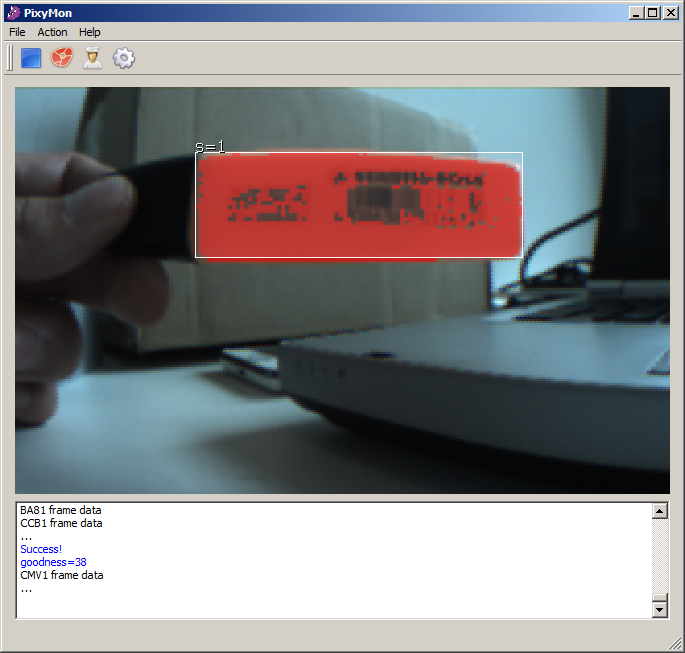
\includegraphics[width=0.7\linewidth]{../../fig/pixy_objekt}
\caption{Pixy erkennt einen Leuchtstift}
\label{fig:pixy_objekt}
\end{figure}